\documentclass[a4paper,11pt]{report}
\usepackage{chuan_math_gkt}
\usetikzlibrary{angles,quotes,intersections,patterns,decorations.pathreplacing}
\chuanexamsetup

\begin{document}
\examfontsize

\examsecret{绝密$\bigstar$启用前}

\examtitle{2020年普通高等学校招生全国统一考试（天津卷）}{数\quad 学}

\noticetitle
\begin{examnotice}
\item 答卷前，考生务必将自己的姓名、准考证号填写在答题卡上. 
\item 回答选择题时，选出每小题的答案后，用铅笔把答题卡上对应题目的答案标号涂黑. 如需改动，用橡皮擦干净后，再选涂其他答案标号. 回答非选择题时，将答案写在答题卡上. 写在本试卷上无效. 
\item 考试结束后，将本试卷和答题卡一并交回. 
\end{examnotice}

\examsection{一、选择题：本大题共9小题，每小题5分，共45分. 在每小题给出的四个选项中，只有一项是符合题目要求的. }
\begin{examquestions}

\item 设全集 $U=\{-3,-2,-1,0,1,2,3\}$，集合 $A=\{-1,0,1,2\}$，$B=\{-3,0,2,3\}$，则 $A\cap(\complement_U B)=$
\fourchoices{$\{-3,3\}$}{$\{0,2\}$}{$\{-1,1\}$}{$\{-3,-2,-1,1,3\}$}
\item 设 $a\in\mathbb R$，则“$a>1$”是“$a^2>a$”的
\twochoices{充分不必要条件}{必要不充分条件}{充要条件}{既不充分也不必要条件}
\item 函数 $y=\dfrac{4x}{x^2+1}$ 的图象大致为
\graphchoices{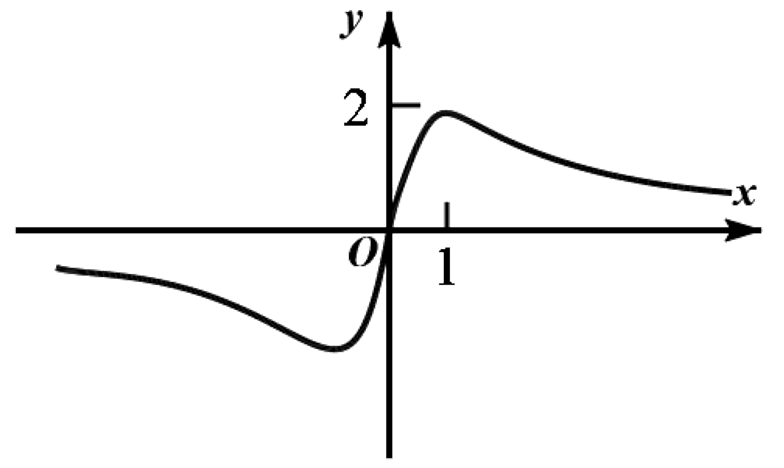
\includegraphics[width=5cm]{figures/2020_tj_q3_A.png}}{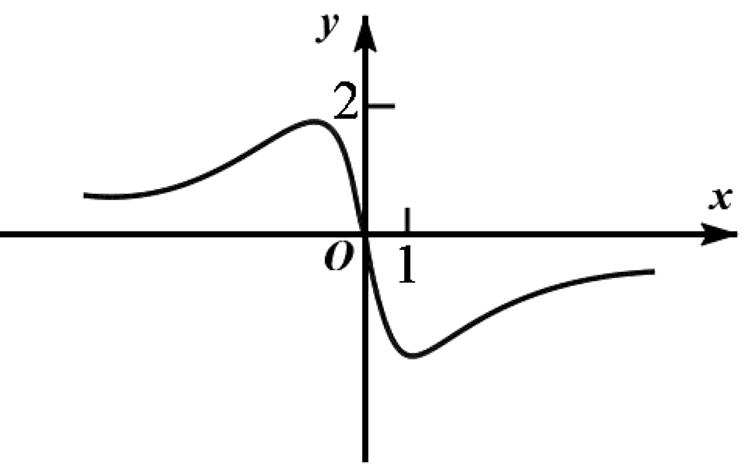
\includegraphics[width=5cm]{figures/2020_tj_q3_B.png}}{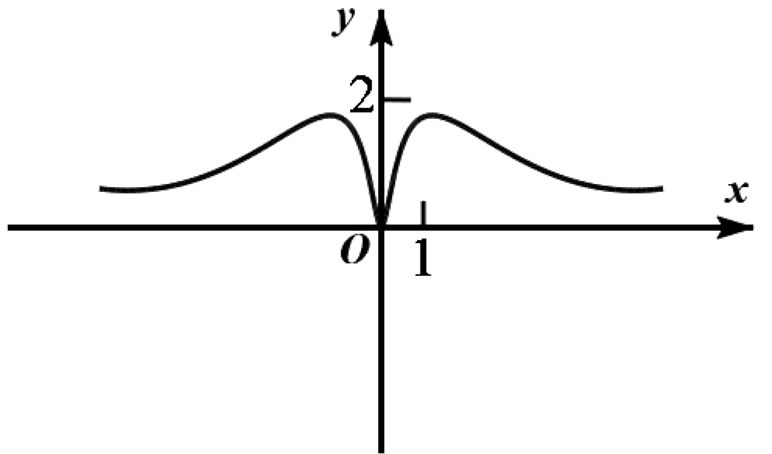
\includegraphics[width=5cm]{figures/2020_tj_q3_C.png}}{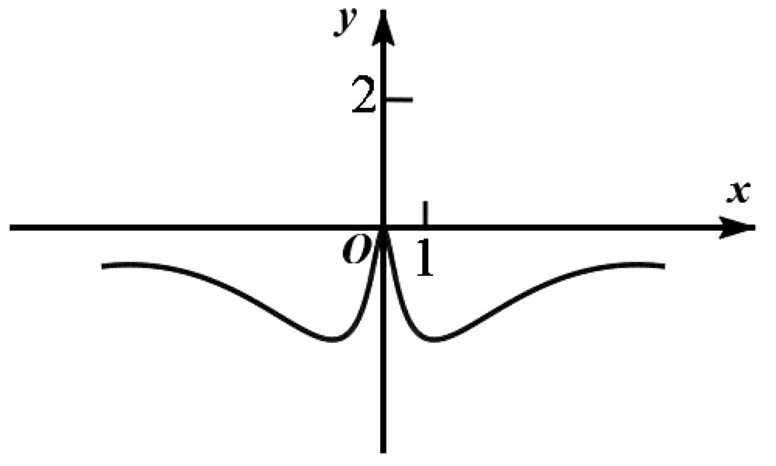
\includegraphics[width=5cm]{figures/2020_tj_q3_D.png}}
\newpage
\item 从一批零件中抽取 $80$ 个，测量其直径（单位：$\mathrm{mm}$），将所得数据分为 $9$ 组：$[5.31,5.33)$, $[5.33,5.35)$, $\ldots$, $[5.47,5.49]$，并整理得到如下频率分布直方图，则在被抽取的零件中，直径落在区间 $[5.43,5.47)$ 内的个数为
\begin{tightcenter}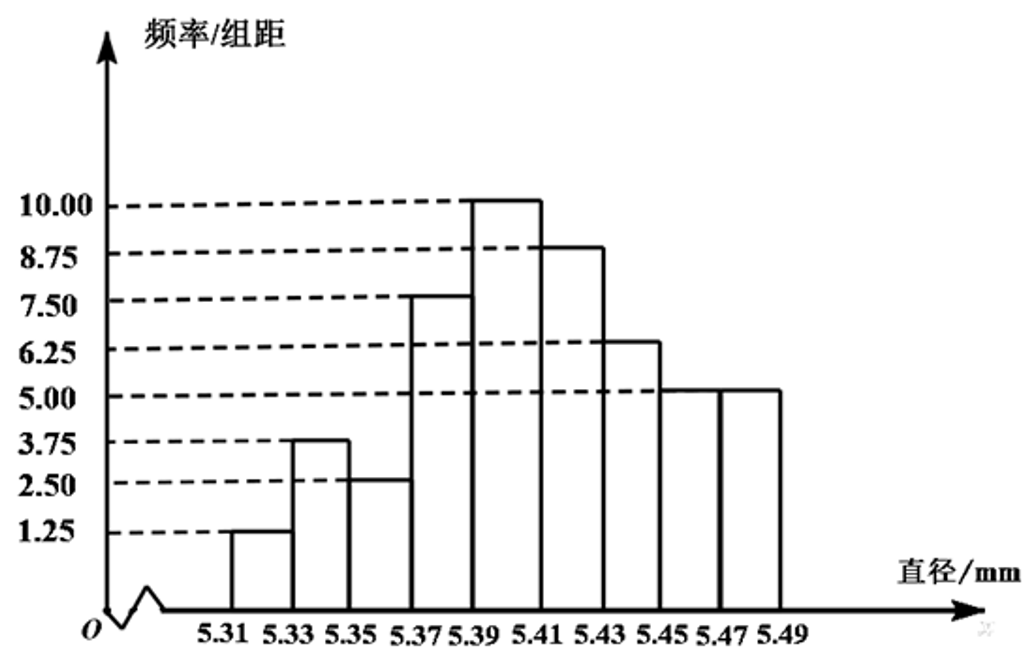
\includegraphics[width=7.6cm]{figures/2020_tj_q4.png}\end{tightcenter}
\fourchoices{$10$}{$18$}{$20$}{$36$}
\item 若棱长为 $2\sqrt3$ 的正方体的顶点都在同一球面上，则该球的表面积为
\fourchoices{$12\pi$}{$24\pi$}{$36\pi$}{$144\pi$}
\item 设 $a=3^{0.7}$，$b=\left(\dfrac13\right)^{-0.8}$，$c=\log_{0.7}0.8$，则 $a,b,c$ 的大小关系为
\fourchoices{$a<b<c$}{$b<a<c$}{$b<c<a$}{$c<a<b$}
\item 设双曲线 $C$ 的方程为 $\dfrac{x^2}{a^2}-\dfrac{y^2}{b^2}=1(a>0,b>0)$，过抛物线 $y^2=4x$ 的焦点和点 $(0,b)$ 的直线为 $l$. 若 $C$ 的一条渐近线与 $l$ 平行，另一条渐近线与 $l$ 垂直，则双曲线 $C$ 的方程为
\fourchoices{\tallchoice{$\dfrac{x^2}{4}-\dfrac{y^2}{4}=1$}}{\tallchoice{$x^2-\dfrac{y^2}{4}=1$}}{\tallchoice{$\dfrac{x^2}{4}-y^2=1$}}{\tallchoice{$x^2-y^2=1$}}
\item 已知函数 $f(x)=\sin\left(x+\dfrac\pi3\right)$. 给出下列结论：

① $f(x)$ 的最小正周期为 $2\pi$；
② $f\left(\dfrac\pi2\right)$ 是 $f(x)$ 的最大值；

③把函数 $y=\sin x$ 的图象上所有点向左平移 $\dfrac\pi3$ 个单位长度，可得到函数 $y=f(x)$ 的图象. 

其中所有正确结论的序号是
\fourchoices{①}{①③}{②③}{①②③}
\item 已知函数 $f(x)=\linsys{x^3,x\geq0,\\-x,x<0}$. 若函数 $g(x)=f(x)-|kx^2-2x|$（$k\in\mathbb R$）恰有 $4$ 个零点，则 $k$ 的取值范围是
\twochoices{\tallchoice{$\left(-\infty,-\dfrac12\right)\cup(2\sqrt2,+\infty)$}}{$\left(-\infty,-\dfrac12\right)\cup(0,2\sqrt2)$}{$(-\infty,0)\cup(0,2\sqrt2)$}{$(-\infty,0)\cup(2\sqrt2,+\infty)$}

\end{examquestions}

\examsection{二、填空题：本大题共6小题，每小题5分，共30分. 试题中包含两个空的，答对1个的给3分，全部答对的给5分. }
\begin{examquestions}[start=10]

\item $\mathrm{i}$ 是虚数单位，复数 $\dfrac{8-\mathrm{i}}{2+\mathrm{i}}=$\blank. 
\item 在 $\left(x+\dfrac2{x^2}\right)^5$ 的展开式中，$x^2$ 的系数是\blank. 
\item 已知直线 $x-\sqrt3y+8=0$ 和圆 $x^2+y^2=r^2(r>0)$ 相交于 $A,B$ 两点. 若 $|AB|=6$，则 $r$ 的值为\blank. 
\item 已知甲、乙两球落入盒子的概率分别为 $\dfrac12$ 和 $\dfrac13$. 假定两球是否落入盒子互不影响，则甲、乙两球都落入盒子的概率为\blank；甲、乙两球至少有一个落入盒子的概率为\blank. 
\item 已知 $a>0$，$b>0$，且 $ab=1$，则 $2a+\dfrac1{2b}+\dfrac8{a+b}$ 的最小值为\blank. 

\noindent\begin{minipage}[t]{0.64\linewidth}
\item 如图，在四边形 $ABCD$ 中，$\angle B=60^\circ$，$AB=3$，$BC=6$，且 $\overrightarrow{AD}=\lambda\overrightarrow{BC}$，$\overrightarrow{AD}\cdot\overrightarrow{AB}=-\dfrac32$，则实数 $\lambda$ 的值为\blank；若 $M,N$ 是线段 $BC$ 上的动点，且 $|MN|=1$，则 $\overrightarrow{DM}\cdot\overrightarrow{DN}$ 的最小值为\blank. 

\end{minipage}\hfill
\begin{minipage}[t]{0.3\linewidth}\vspace{0em}\centering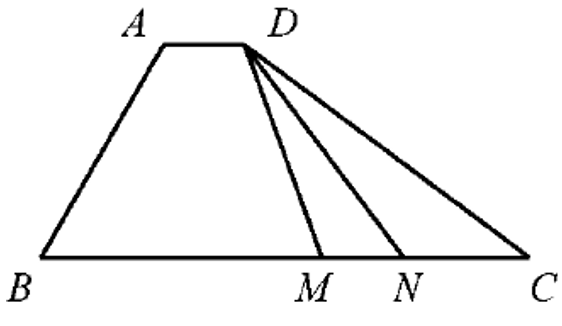
\includegraphics[width=\linewidth]{figures/2020_tj_q15.png}\end{minipage}


\end{examquestions}

\examsection{三、解答题：本大题共5小题，共75分. 解答应写出文字说明、证明过程或演算步骤. }
\begin{examanswers}[start=16]

\item（14分）

在 $\triangle ABC$ 中，角 $A,B,C$ 所对的边分别为 $a,b,c$. 已知 $a=2\sqrt2$，$b=5$，$c=\sqrt{13}$. 

\subq{（1）}{求角 $C$ 的大小；}

\subq{（2）}{求 $\sin A$ 的值；}

\subq{（3）}{求 $\sin\left(2A+\dfrac\pi4\right)$ 的值. }

\item（15分）

如图，在三棱柱 $ABC-A_1B_1C_1$ 中，$CC_1\perp$ 平面 $ABC$，$AC\perp BC$，$AC=BC=2$，$CC_1=3$，点 $D,E$ 分别在棱 $AA_1$ 和棱 $CC_1$ 上，且 $AD=1$，$CE=2$，$M$ 为棱 $A_1B_1$ 的中点. 

\noindent\begin{minipage}[t]{0.64\linewidth}
\subq{（1）}{求证：$C_1M\perp B_1D$；}

\subq{（2）}{求二面角 $B-B_1E-D$ 的正弦值；}

\subq{（3）}{求直线 $AB$ 与平面 $DB_1E$ 所成角的正弦值. }
\end{minipage}\hfill
\begin{minipage}[t]{0.23\linewidth}\vspace{-1.2em}\centering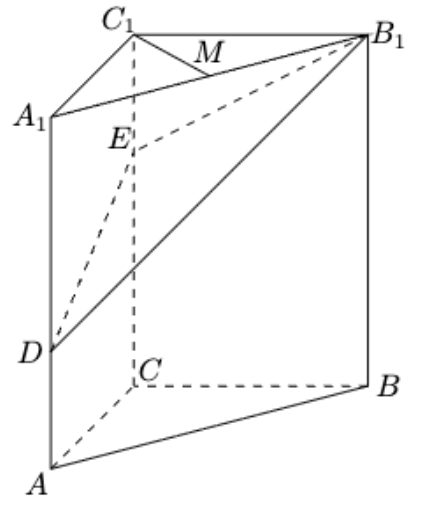
\includegraphics[width=\linewidth]{figures/2020_tj_q17.png}\end{minipage}

\item（15分）

已知椭圆 $\dfrac{x^2}{a^2}+\dfrac{y^2}{b^2}=1(a>b>0)$ 的一个顶点为 $A(0,-3)$，右焦点为 $F$，且 $|OA|=|OF|$，其中 $O$ 为原点. 

\subq{（1）}{求椭圆方程；}

\subq{（2）}{已知点 $C$ 满足 $3\overrightarrow{OC}=\overrightarrow{OF}$，点 $B$ 在椭圆上（$B$ 异于椭圆的顶点），直线 $AB$ 与以 $C$ 为圆心的圆相切于点 $P$，且 $P$ 为线段 $AB$ 的中点，求直线 $AB$ 的方程. }

\item（15分）

已知 $\{a_n\}$ 为等差数列，$\{b_n\}$ 为等比数列，$a_1=b_1=1$，$a_5=5(a_4-a_3)$，$b_5=4(b_4-b_3)$. 

\subq{（1）}{求 $\{a_n\}$ 和 $\{b_n\}$ 的通项公式；}

\subq{（2）}{记 $\{a_n\}$ 的前 $n$ 项和为 $S_n$，求证：$S_nS_{n+2}<S_{n+1}^2(n\in\mathbb N^*)$；}

\subq{（3）}{对任意正整数 $n$，设 $c_n=\linsys{\dfrac{(3a_n-2)b_n}{a_na_{n+2}},\quad n\text{为奇数},\\\dfrac{a_{n-1}}{b_{n+1}},\quad n\text{为偶数}}$，求 $\{c_n\}$ 的前 $2n$ 项和. }

\item（16分）

已知函数 $f(x)=x^3+k\ln x(k\in\mathbb R)$，$f'(x)$ 为 $f(x)$ 的导函数. 

\subq{（1）}{当 $k=6$ 时，}

\subq{（i）}{求曲线 $y=f(x)$ 在点 $(1,f(1))$ 处的切线方程；}

\subq{（ii）}{求函数 $g(x)=f(x)-f'(x)+\dfrac9x$ 的单调区间和极值；}

\subq{（2）}{当 $k>-3$ 时，求证：对任意的 $x_1,x_2\in[1,+\infty)$，且 $x_1>x_2$，有 $\dfrac{f'(x_1)+f'(x_2)}2>\dfrac{f(x_1)-f(x_2)}{x_1-x_2}$. }
\end{examanswers}

\end{document}
